\section{New Capabilities}
\label{s:capabilities}
\ma{I don't think we need to change this. 'New Capabilities' seems fine}

\begin{figure}
    \centering
    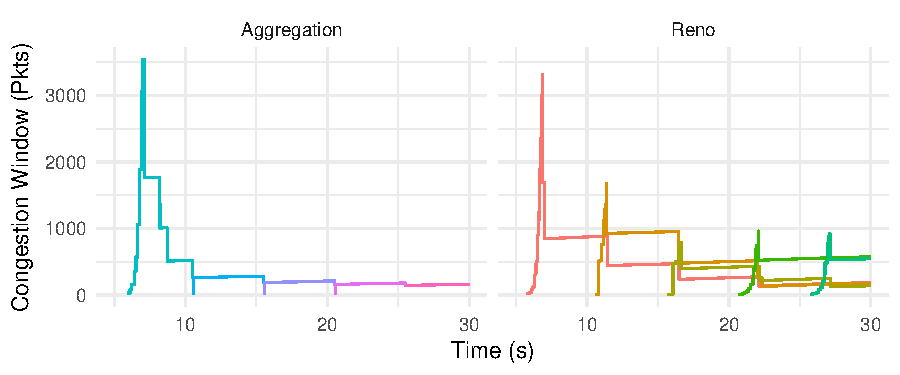
\includegraphics[width=\columnwidth]{img/stair}
    \caption{5 20-second iperf flows with 10 second staggered starts. While Reno (right) must individually probe for bandwidth for each new connection, an aggregating congestion controller is able to immediately set the connection's congestion window to the fair share value.}
    \label{fig:cap:agg}
\end{figure}
\begin{figure*}[t!]
    \centering
    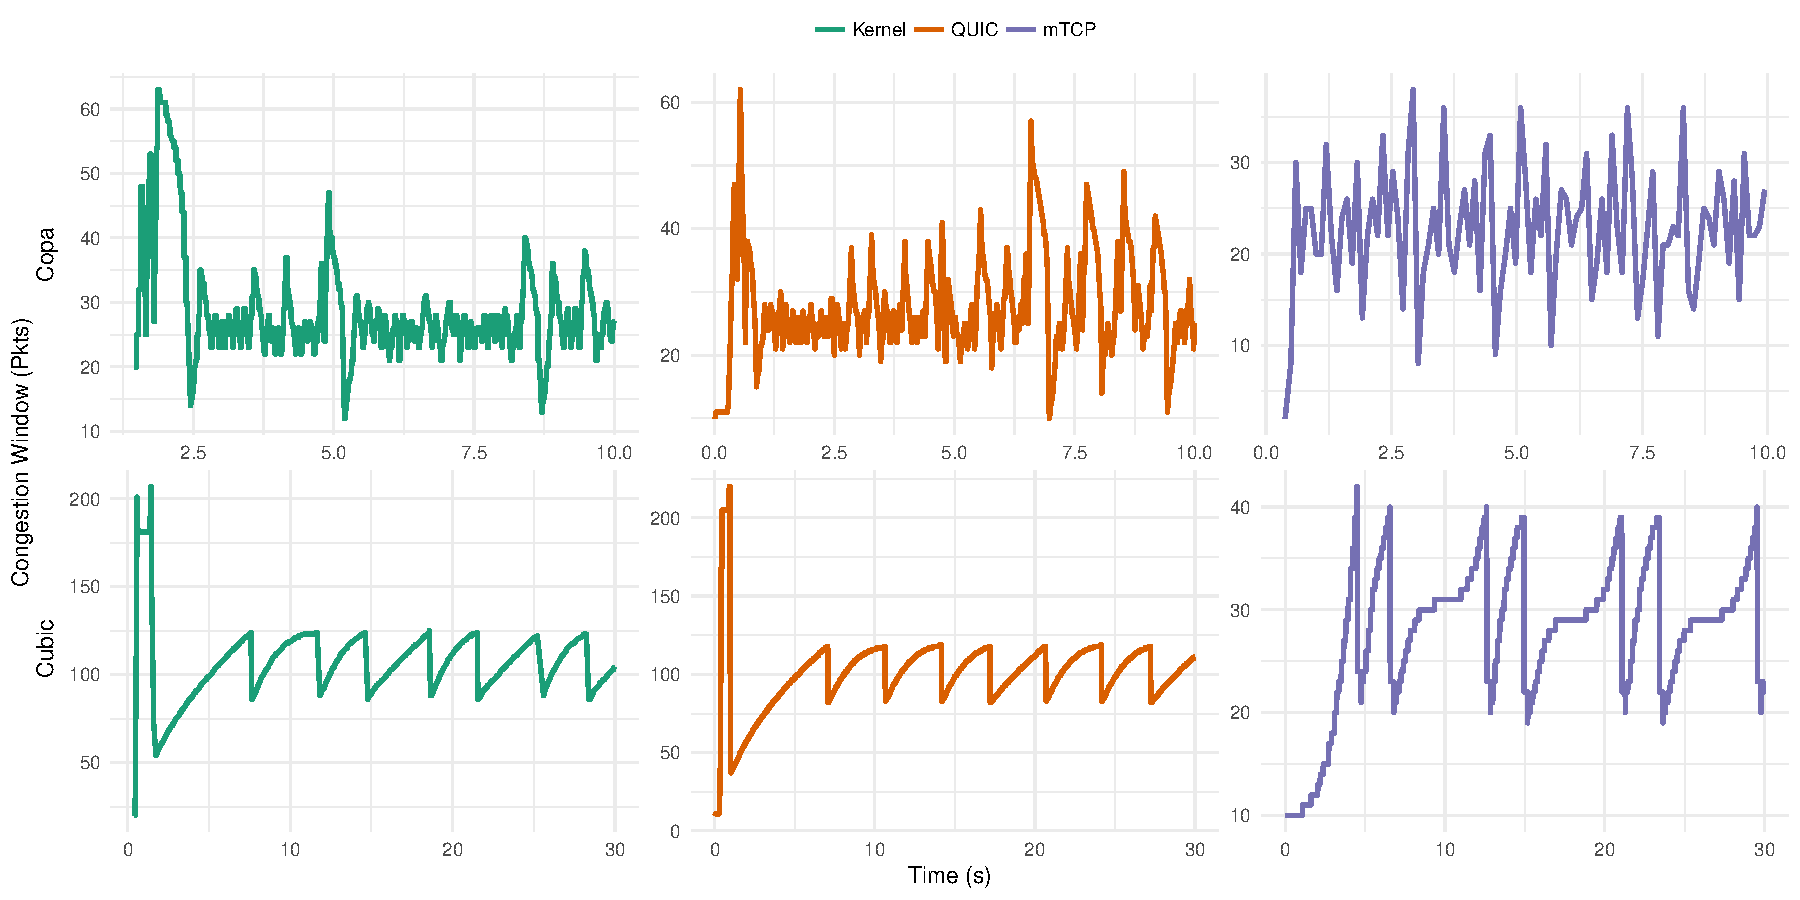
\includegraphics[width=2\columnwidth]{img/new-wora}
    \caption{Comparison of the same CCP implementation of Cubic and Copa run on three different datapaths. Copa is run on a 12 Mbps link for all three datapaths. For Cubic, we use a 48 Mbps link on the QUIC and kernel datapaths. mTCP did not exhibit stable behavior at higher bandwidths, so we ran mTCP at 12 Mbps; this is why the congestion window is lower.}\label{fig:datapaths:wora}
\end{figure*}

We present four new capabilities enabled by CCP: congestion control algorithms that leverage user-space programming libraries, rapid development and testing of algorithms, congestion control for flow aggregates, and the ability to write an algorithm once and run it on multiple datapaths.

\subsection{Sophisticated Congestion Control Algorithms}
\label{s:capabilities:algs}

CCP makes it possible to use sophisticated user-space libraries, such as libraries for signal processing, machine learning, etc. to implement congestion control algorithms.

One example is Nimbus~\cite{nimbus}, a new congestion control algorithm that detects whether the cross traffic at a bottleneck link is  elastic (buffer-filling) or not, and uses different control rules depending on the outcome. The Nimbus algorithm involves sending traffic in an asymmetric sinusoidal pulse pattern and using the sending and receiving rates measured over an RTT to produce a time-series of cross-traffic rates. The method then computes the FFT of this time-series and infers elasticity if the FFT at particular frequencies is large.

The implementation of Nimbus uses CCP to configure the datapath to report the sending and receiving rates periodically (e.g., every 10 ms), maintains a time-series of the measurements in user-space, and performs FFT calculations using a FFT library in Rust~\cite{}. 

Although it is possible to implement such algorithms directly in the datapath, it would be significantly more difficult. For instance, one would need to implement the FFT operations with fixed-point arithmetic. Moreover, implementing the algorithm outside the datapath using CCP allows for a tighter development-testing loop than writing kernel code.

%such sinusoidal pulses within the datapath, but computing the FFT is unlikely to be practical both due to the timing requirements of the ACK clock as well as the difficulty of performing complex calculations in restrictive programming environments such as the kernel. Moreover, implementing the transmitter outside the datapath in CCP allowed for a tighter development-testing loop than writing kernel code.
%Figure~\ref{fig:capabilities:nimbus-example} shows this pulse pattern and the result of the FFT computation.

We anticipate that in the future, CCP will enable the use of other similarly powerful but computationally-intensive methods such as neural networks.

%such algorithmic technique~\cite{nimbus} uses CCP to compute Fourier transforms on estimates of cross traffic and infer whether it is elastic (buffer-filling) or not.
%A key component of this technique involves sending traffic in an asymmetric sinusoidal pulse pattern and using the sending and receiving rates measured over an RTT to produce a time-series of cross-traffic rates. The method then computes the FFT of this series and infers elasticity if the FFT at particular frequencies is large.


% CCP enables a broad new class of congestion control algorithms.
% Until now, because congestion control has been embedded in the datapath,
% algorithms have been strictly tied to the ACK clock.
% As a result, as data rates rise, algorithms have less time to make decisions,
% which naturally restricts the computation an algorithm can perform.
% By contrast, CCP algorithms are decoupled from the ACK clock.
% Although congestion signals must still be acquired and summarized at ever-faster rates, CCP algorithms can amortize computation across different time scales, and use sophisticated data structures and computations that may be unwise on datapaths like the kernel.


% In principle, it may be possible to implement such sinusoidal pulses within the datapath, but computing the FFT is unlikely to be practical both due to the timing requirements of the ACK clock as well as the difficulty of performing complex calculations in restrictive programming environments such as the kernel. Moreover, implementing the transmitter outside the datapath in CCP allowed for a tighter development-testing loop than writing kernel code.
% %Figure~\ref{fig:capabilities:nimbus-example} shows this pulse pattern and the result of the FFT computation.
% We anticipate that in the future, CCP will enable the use of other similarly powerful but computationally-intensive methods such as neural networks.

\subsection{Velocity of Development}
\label{s:capabilities:velocity}

Copa~\cite{copa} is a recently proposed model-based congestion control algorithm that seeks to maintain a target rate that is inversely proportional to the queuing delay, estimated as the difference of the current RTT and the minimum RTT.
%Under three network models, this is shown to provide quantifiably low delay, and fair and efficient allocation of bandwidth.
It is robust to non-congestive loss, buffer-bloat, and unequal propagation delays. It includes mechanisms to provide TCP competitiveness, accurate minimum RTT estimation, and imperfect pacing.

The authors of Copa used CCP to implement Copa recently, and in the process discovered a small bug that produced an erroneous minimum RTT estimate due to ACK compression. They solved this problem with a small modification to the Copa datapath program,
and in a few hours were able to improve the performance of their earlier user-space implementation. The improvement is summarized here:

\begin{tabular}{c|c|c}
    Algorithm & Throughput & Mean queue delay \\
    \hline
    Copa (UDP) & 1.3 Mbit/s & 9 ms\\
    Copa (CCP-Kernel) & 8.2 Mbit/s  & 11 ms\\
\end{tabular}

\smallskip
After the ACK compression bug was fixed in the CCP version, Copa achieves higher throughput on a Mahimahi link with 25 ms RTT and 12 Mbit/s rate while maintaining low mean queueing delay. Because of ACK compression, the UDP version over-estimates the minimum RTT by $5\times$.

\subsection{Flow Aggregation}
\label{s:capabilities:agg}

% from nimbus nsdi submission's intro
Congestion control on the Internet is performed by individual TCP connections. Each connection independently probes for bandwidth, detects congestion on its path, and reacts to it.
This per-connection paradigm for congestion control is a poor fit in many modern traffic control scenarios where a large number of nodes exchange traffic between a few sites.
Examples include: traffic between different datacenters~\cite{b4, swan}; traffic between campuses of an organization; large-scale data backups from an organization to an external site; etc.

We focus on the per-host aggregation proposed by the
Congestion Manager two decades ago~\cite{cm}. We used CCP to develop a
host-level aggregate controller that maintains a single aggregate window or rate
for a group of flows and allocates that to individual flows---all with no
  changes to the non-CCP parts of the datapath.

%
%Since CCP has visibility into all the flows in the system, it is uniquely positioned as a platform on which users can implement aggregate congestion control.
%In fact, we make a small modification to CCP to support flow aggregation and show that a proof-of-concept implementation can reduce average flow completion times by \an{XXX}\%.

\paragrapha{Interface} In addition to the \texttt{create()} and \texttt{onReport()} event handlers, we introduce two new APIs for aggregate congestion controllers: \texttt{create\_subflow()} and \texttt{aggregateBy()}.
CCP uses \texttt{aggregateBy()} to classify new connections into aggregates. Then, it calls either the existing \texttt{create()} handler in the case of a new aggregate, or the \texttt{create\_subflow()} handler in the case of an already active one.

These handlers are natural extensions of the existing per-flow API; we implemented API support for aggregation in $80$ lines of code in our Rust CCP implementation (\S\ref{sec:eval}).
Algorithms can aggregate flows using the connection 5-tuple, passed as an argument to \texttt{aggregateBy()}.

As a proof of concept, we implement an algorithm which simply aggregates all flows on each of the hosts's interfaces into one aggregate and assigns the window in equal portions to each sub-flow.
Figure~\ref{fig:cap:agg} shows the aggregator instantaneously apportioning equal windows to each flow in its domain.

 
\subsection{Write-Once, Run-Anywhere}
\label{s:capabilities:wora}
\label{s:datapaths:eval}

Correct implementation of congestion control algorithms, especially increasingly complicated recent work, is a significant undertaking.
As a result, new algorithms are often implemented in a single datapath and new datapaths have very few algorithms implemented. 
CCP enables algorithm designers to focus on building and testing a single solid implementation of their algorithm that users can then run on any (supported) datapath. 

To exhibit this capability, we ran the same implementation of both Cubic (not previously implemented in mTCP) and Copa (\S\ref{s:capabilities:velocity}, not previously implemented in any widely-used datapath) on the three datapaths and plot the congestion window evolution over time in Figure~\ref{fig:datapaths:wora}.

As expected, the congestion window naturally evolves differently on each datapath, but the characteristic shapes of both algorithms are clearly visible. Copa uses triangular oscillations around an equilibrium of 1 BDP worth of packets (22 in this case), periodically draining the queue in an attempt to estimate the minimum RTT.